\chapter{Kiến thức nền tảng}
\section{Học máy}

Học máy được sử dụng rất nhiều trong thị giác máy tính. Trước khi xem xét các nhiệm vụ liên quan đến hình ảnh, nhóm sẽ có một cái nhìn sơ lược về những điều cơ bản trong học máy.\\

Học máy đã xuất hiện như một công cụ hữu ích với khả năng tự học hỏi dựa trên dữ liệu mà không cần phải lập trình cụ thể. Những năm gần đây, khi mà khả năng tính toán của các máy tính được nâng lên một tầm cao mới và lượng dữ liệu khổng lồ được thu thập bởi các hãng công nghệ lớn, học máy đã tiến thêm một bước dài và ngày càng phổ biến với khả năng ngày càng mạnh mẽ.


\subsection{Phân loại các thuật toán học máy}

Theo phương thức học, các thuật toán học máy thường được chia thành các nhóm khác nhau: học có giám sát, học không giám sát, học bán giám sát...\\

\textbf{Học có giám sát} là nhóm phổ biến nhất trong các thuật toán học máy. Nó là thuật toán dự đoán đầu ra của một dữ liệu mới dựa trên các cặp (dữ liệu, nhãn) đã biết từ trước. Ví dụ trong vấn đề nhận diện vật thể, chúng ta sẽ sử dụng dữ liệu đã được đánh dấu vị trí và lớp của các vật thể riêng biệt để huấn luyện. Sau khi học xong, thuật toán có thể dự đoán lớp và vị trí của những dữ liệu mới. \textit{Phân lớp} và \textit{hồi quy} là hai loại chính trong học có giám sát. Trong phân lớp, thuật toán sẽ dự đoán các lớp chính xác của dữ liệu mới dựa trên dữ liệu huấn luyện. Trong hồi quy, thay vì chia thành các nhóm thì đầu ra là một giá trị cụ thể. Gần đây, Microsoft có ứng dụng dự đoán giới tính và tuổi dựa trên khuôn mặt, thì phần dự đoán giới tính có thể coi là thuật toán phân lớp, phần dự đoán tuổi có thể coi là thuật toán hồi quy.\\

Với \textbf{học không giám sát}, chúng ta không biết được outcome hay nhãn mà chỉ có dữ liệu đầu vào. Sau đó, dựa vào cấu trúc dữ liệu để thực hiện một công việc nào đó, có thể là phân nhóm, dự đoán xu hướng của thị trường ... Các bài toán trong học không giám sát cũng được phân loại, trong đó bài toán \textit{phân nhóm} thực hiện việc phân nhóm toàn bộ dữ liệu thành các nhóm nhỏ dựa trên sự liên quan về dữ liệu trong mỗi nhóm. Ngoài ra, còn có bài toán khi chúng ta muốn khám phá quy luật dựa trên nhiều dữ liệu đã cho trước. Chẳng hạn như những khác hàng mua quần thường có xu hướng mua thêm thắt lưng, hay bia sẽ được tiêu thụ nhiều hơn vào thời gian hè..., từ đó tạo ra hệ thống gợi ý khách hàng, thúc đẩy nhu cầu mua sắm.

\subsection{Tính tổng quát}

Bởi vì dữ liệu huấn luyện không thể bao hàm tất cả mọi trường hợp có thể của dữ liệu đầu vào, do đó, thuật toán học phải có tính tổng quát để có thể xử lí các dữ liệu mới. Một mô hình quá đơn giản sẽ không thể tạo ra được kết quả mong muốn với độ chính xác thấp, còn nếu mô hình quá phức tạp có thể dẫn đến tình trạng quá khớp. Do vậy, tính tổng quát của mô hình rất quan trọng trong việc ứng dụng thực tế.\\

Độ hiệu quả của thuật toán có thể được đánh giá dựa trên hàm mất mát(loss). Hàm mất mát được sử dụng để lượng giá giá trị đầu ra với giá trị thực tế là bao nhiêu. Nếu giá trị lỗi lớn, nghĩa là mô hình của chúng ta chưa thực hiện tốt, độ lỗi càng nhỏ càng thể hiện mô hình đang học tốt hơn. Mặt khác, cần phải quan tâm tới tính tổng quát của mô hình như đã nhắc đến ở trên. Mục tiêu trong giai đoạn huấn luyện chính là tìm cực tiểu của hàm mất mát này.

\section{Neural Networks}

Mạng nơ-ron được được phát minh cách đây khá lâu, nhưng mãi đến gần đây nó mới bắt đầu trở nên phổ biến và được sử dụng rộng rãi. Nguyên nhân là do mạng nơ-ron cần có thiết bị tính toán mạnh mẽ và lượng dữ liệu đủ lớn để huấn luyện. Trước kia, công nghệ phát triển chưa đạt đến trình độ để tạo ra những thiết bị hỗ trợ tính toán cao và lượng dữ liệu thu thập được còn quá ít nên đã kìm hãm sự phát phát triển của mạng nơ-ron. Công nghệ ngày càng phát triển theo thời gian, nhu cầu tính toán ngày càng tăng đã tạo động lực thúc đẩy phát minh ra những thiết bị tính toán ngày càng mạnh mẽ. Thế giới ngày càng trở nên số hóa, các thiết bị số ngày một nhiều, do đó đã góp phần tạo nên một lượng dữ liệu rất lớn. Chính hai điều kiện trên đã góp phần tạo điều kiện cho mạng nơ-ron ngày nay trở nên phát triển và khá phổ biến dưới cái tên "deep learning" nhằm nhấn mạnh những kiến trúc sâu được tạo ra bằng cách chồng các lớp lên nhau.

Mạng nơ-ron là giải thuật học máy được sử dụng nhiều. Và nó cũng là nền tảng để nghiên cứu giải quyết bài toán phát hiện vật thể trong không gian 2 hiều, vì cho đến hiện nay, các mô hình tốt nhất vẫn sử dụng kiến thức từ mạng nơ-ron nhiều lớp. Mạng nơ-ron ngày nay được ứng dụng khá rộng rãi trong nhiều lĩnh vực như thị giác máy tính, nhận diện giọng nói, xử lí ngôn ngữ tự nhiên.Đầu tiên, chúng ta sẽ tìm hiểu cách hoạt động của mạng nơ-ron.

\subsection{Nơ-ron nhân tạo}

Mạng nơ-ron ban đầu được gọi là mạng nơ-ron nhân tạo, bảo vì chúng đã được phát triển dựa trên chức năng thần kinh của bộ não con người. Nghiên cứu tiên phong là của 2 nhà khoa học McCulloch và Pitts. 

\begin{figure}[H]%
    \centering
    \subfloat[A biological neuron]{{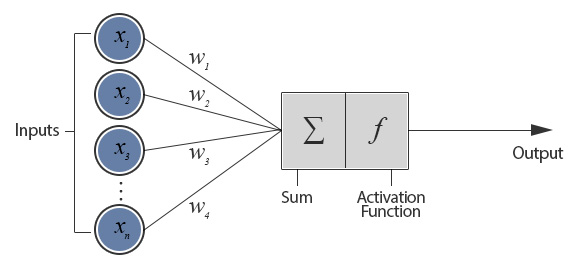
\includegraphics[height=4cm,width=6cm]{image/chapter3_ann} }}%
    \qquad
    \subfloat[Artificial neuron]{{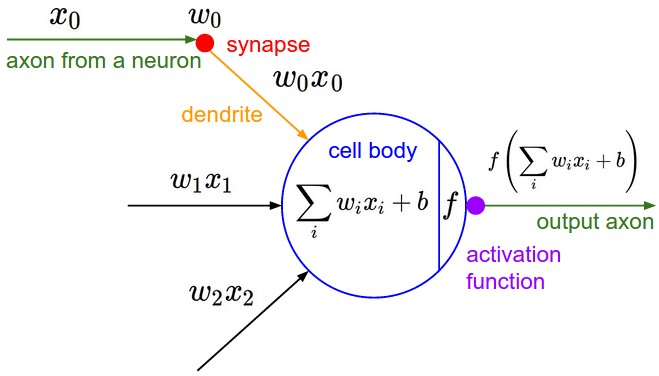
\includegraphics[height=4cm,width=6cm]{image/chapter3_ann_2} }}%
    \caption{A cartoon drawing of a biological neuron (left) and its mathematical model (right).}%
    \label{fig:neuron}%
\end{figure}



Một nơ-ron nhân tạo dựa trên mô hình của McCulloch-Pitts được thể hiện trên hình \ref{fig:neuron}. Nơ-ron nhận n đầu vào với các tham số $x_1, x_2, ...x_i$. Nơ-ron cũng có n trọng số $w_1, w_2, ...w_i$. Những trọng số này thường có một bias với giá trị cố định. Các giá trị đầu vào của nơ-ron kết hợp tuyến tính với các trọng số và được tính tổng lại. Tổng đó sẽ được đưa vào như là input của hàm kích hoạt $f$ (\textbf{activation function}) và tạo ra giá trị output của nơ-ron. Trong lịch sử, lựa chọn phổ biến cho hàm kích hoạt đó là hàm \textbf{sigmoid}, nó lấy input (tổng của các tín hiệu được truyền tới) và nén lại để output sẽ nằm giữa khoảng từ 0 đến 1. Ý tưởng chính ở đây là các giá trị trọng số có thể học được, dựa vào đó đưa ra ouput phù hợp với mỗi input.\\

\begin{center}
	\begin{equation}
		y = f(s) = f(\displaystyle \sum_{i=1}^n(w_ix_i+b_i))
	\end{equation}
\end{center}

Một nơ-ron đơn giống như là một phân loại tuyến tính. Chúng ta có thể thấy với nó sẽ "thích" (kết quả của hàm kích hoạt sẽ gần bằng 1) hoặc "không thích" (kết quả của hàm kích hoạt sẽ gần bằng 0) với giá trị input cụ thể. 

\subsection{Activation function types}

Hàm activation $f$ sẽ nhận vào một số và thực hiện tính toán để xác định output của mỗi nơ-ron. Do vậy, việc chọn hàm activation là quan trọng để có thể tạo ra một mạng hiệu quả. Các nhà nghiên cứu đã sớm nhìn thấy  các nơ-ron và các hệ thống tuyến tính khác sẽ không thể giải quyết được các bài toán không khả phân, ví dụ như bài toán XOR.  Việc thêm nhiều lớp tuyến tính cũng sẽ không thay đổi được vấn đè, bởi vì một mạng kết hợp của nhiều nơ-ron tuyến tính thì nó vẫn duy trì tính tuyến tính. \\

Do vậy, cách đơn giản và hiệu quả để tạo ra một mạng phi tuyến chính là chọn hàm activation phi tuyến. Các hàm activation thường được dùng như  \textit{hàm sigmoid, hàm tanh, hàm ReLU (rectified linear units)}.\\

\begin{center}
   \begin{figure}[htp]
   \begin{center}
     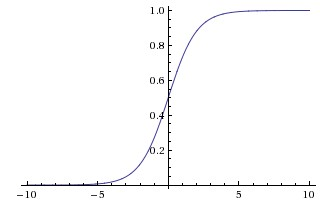
\includegraphics[scale=.5]{image/sigmoid}
    \end{center}
    \caption{Sigmoid function}
    \label{fig:sigmoid}
    \end{figure}
\end{center}

\textbf{Sigmoid}: Sigmoid là một hàm phi tuyến và có công thức toán học: \textbf{$\phi(x) = \dfrac{1}{1+e^x}$} với đạo hàm $f'(x) = f(1-f)$ với đồ thị được thể hiện ở hình trên. Theo như đã nói trước đây, hàm sigmoid sẽ nhận giá trị input và nén chúng thành những giá trị nằm trong khoảng 0 và 1.Trên thực tế, những số âm rất lớn sẽ trở thành 0, những số dương rất lớn sẽ trở thành 1. Do vậy, gần đây hàm sigmoid hiếm khi được sử dụng với các nhược điểm:
\begin{itemize}
	\item Sigmoid mang tính bão hòa và sẽ triệt tiêu đạo hàm. Một thuộc tính không mong muốn của sigmoid đó là khi giá trị của nó tiến về gần 0 hoặc 1, thì đạo hàm tại những vùng đó hầu hết sẽ là 0. Vì trong quá trình backpropagation (sẽ nói đến sau), giá trị đạo hàm này sẽ được nhân với đạo hàm của ouput cho toàn bộ cổng ra. Do đó, nếu giá trị đạo hàm tại đây quá nhỏ, nó sẽ triệu tiêu đạo hàm và hầu như sẽ không có tín hiệu nào được truyền đi, như vậy việc học để cập nhật trọng số sẽ không được thực hiện.
	\item Giá trị của hàm sigmoid sẽ không zero-centered. Nghĩa là nếu giá trị input đến nơ-ron là luôn dương (x>0 với mọi phần tử trong $f = w^Tx+b)$ thì đạo hàm của trọng số $w$ trong suốt quá trình backpropagation sẽ luôn cùng âm hoặc cùng dương. Điều này có thể sẽ dẫn đến việc zig-zaging trong quá trình cập nhật trọng số.
	\item Chi phí tính toán khá lớn.
	
\end{itemize}

\begin{center}
   \begin{figure}[htp]
   \begin{center}
     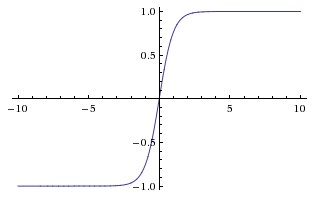
\includegraphics[scale=.5]{image/tanh}
    \end{center}
    \caption{Tanh function}
    \label{fig:tanh}
    \end{figure}
\end{center}

\textbf{Tanh}. Hàm tanh phi tuyến được thể hiện ở hình trên với công thức $tanh(x)=\dfrac{1-e^{-2x}}{1+e^{-2x}} $. Nó sẽ nén các giá trị vào khoảng [-1,1]. Cũng giống như sigmoid nơ-ron, nó cũng sẽ mang tính bão hòa và triệt tiêu đạo hàm. Chi phí tính toán của hàm tanh cũng khá lớn.

\begin{center}
   \begin{figure}[htp]
   \begin{center}
     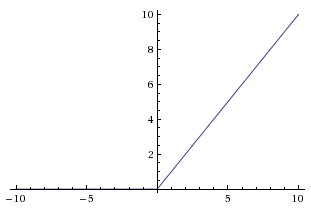
\includegraphics[scale=.5]{image/relu}
    \end{center}
    \caption{ReLU function}
    \label{fig:tanh}
    \end{figure}
\end{center}

\textbf{ReLU}. Hiện nay, hàm ReLU trở nên khá phổ biến, được tính theo công thức $f(x)=max(0,x)$. Với hàm ReLU:
\begin{itemize}
	\item Nó tăng rất nhiều tốc độ tính toán và sự hội tụ của hàm tối ưu nếu so sánh với hàm sigmoid, tanh.
	\item Nếu so sánh về chi phí tính toán của hàm sigmoid, tanh thì hàm ReLU được thực hiện một cách đơn giản, với chi phí thấp.
	\item Ngược lại, sẽ có các thành phần có thể chết và không thể hồi phục trong quá trình luyện. Nếu có một giá trị đạo hàm lớn thì một nơ-ron ReLU có thể làm cho trọng số của phần tử lớn nhất sẽ được cập nhật, còn lại sẽ không bao giờ được cập nhật với bất kì dữ liệu nào nữa. 
\end{itemize}

Vẫn còn nhiều hàm kích hoạt nhưng nhóm chỉ chủ yếu tìm hiểu các loại trên.

\subsection{Multi-layer networks}

\begin{center}
    \begin{figure}[htp]
    \begin{center}
     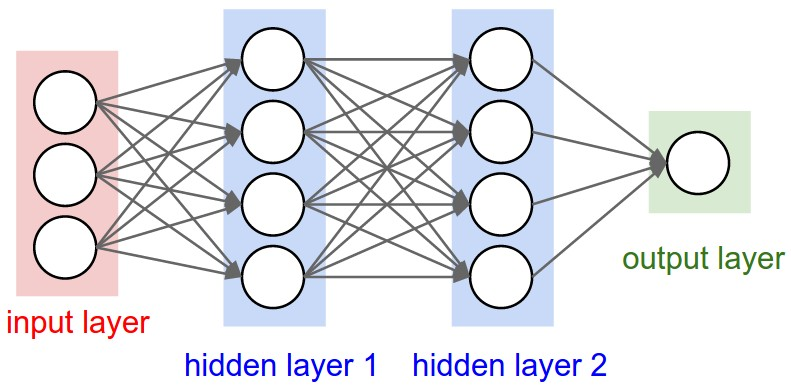
\includegraphics[scale=.4]{image/neural_net2}
    \end{center}
    \caption{A 3-layer neural network}
    \label{fig:multilayer}
    \end{figure}
\end{center}

Mạng nơ-ron là sự kết hợp của nhiều nơ-ron kết nối với nhau. Nói cách khác, thì giá trị đầu ra của một vài nơ-ron sẽ là giá trị đầu vào của những nơ-ron khác. Thay vì một kiến trúc vô định hình các kết nối của các nơ-ron, mạng nơ-ron thường được tổ chức thành các lớp phân biệt của các nơ-ron với nhau. Đối với một mạng nơ-ron thông thường, thì kiểu thường thấy sẽ là fully-connected đối với các nơ-ron giữa hai lớp kề nhau, nhưng những nơ-ron trong cùng một lớp sẽ không có kết nối với nhau. Tính chất của lớp fully-connected là mỗi nơ-ron có số trọng số bằng với số nơ-ron của lớp đứng liền trước nó.\\

Một multi-layer network điển hình bao gồm 3 kiểu lớp, lớp đầu vào, lớp ẩn (hidden layer) và lớp output. Lớp đầu vào thường chỉ truyền dữ liệu đi và không sửa đổi nó. Hầu hết quá trình tính toán xảy ra tại các lớp ẩn. Cuối cùng, lớp đầu ra chuyển giá trị từ các hàm activation của lớp ẩn thành output mong muốn, chẳng hạn là kết quả phân lớp. Một multi-layer network sẽ có ít nhất một lớp ẩn để thực hiện việc tính toán.\\

\subsection{Backpropagation}

Một mạng nơ-ron được huấn luyện chính là việc chọn lựa các trọng số cho tất cả các nơ-ron có trong mạng , từ đó đạt được xấp xỉ các mục tiêu giá trị đầu ra từ những đầu vào đã biết. Việc tìm các trọng số phù hợp của một mạng multi-layer là một công việc khó. Và giải thuật lan truyền ngược(backpropagation) chính là giải pháp phù hợp và hiệu quả để tìm các trọng số. Backpropagation cổ điển sử dụng phương pháp gradient descent như là hàm tối ưu. Gradient descent có thể tốn khá nhiều thời gian và không đảm bảo sẽ tìm được cực tiểu toàn cục của hàm mất mát (loss function), nhưng với việc điều chỉnh phù hợp, nó đủ tốt để có thể ứng dụng trong thực tế.\\

Trong giai đoạn đầu, vector input sẽ được truyền qua mạng nơ-ron, gọi là feedforward. Trước đó, các trọng số của mạng nơ-ron sẽ được khởi tạo giá trị. Output nhận được của mạng nơ-ron sẽ được so sánh với output thật sự, được biết trước ở dữ liệu huấn luyện, bằng việc sử dụng hàm mất mát. Đạo hàm của hàm mất mát sẽ được tính và cũng có thể gọi là giá trị lỗi. Khi sử dụng \textbf{mean squared error (MSE)} như là hàm mất mát, thì giá trị lỗi được hiểu đơn giản là sự khác biệt giữa output hiện tại và output thật sự. \\

Giá trị lỗi sẽ được lan truyền ngược lại trong mạng để tính giá trị lỗi tại các lớp ẩn, gọi là lan truyền ngược(backpropagation). Giá trị lỗi tại các lớp ẩn có thể được tính bằng cách vận dụng đạo hàm của hàm hợp. Cuối cùng, các trọng số của mạng sẽ được cập nhật bằng việc trừ đi một lượng dựa vào tốc độ học (learning rate). Learning rate có thể được đặt cố định hoặc động. Sau khi các trọng số được cập nhật, thuật toán sẽ thực thi lại với dữ liệu đầu vào còn lại trong tập dữ liệu huấn luyện đến khi việc cập nhật trọng số không gây ảnh hưởng nhiều đến giá trị của nó hoặc  dựa vào số lượng dữ liệu trong tập huấn luyện. \\

Trong mô tả ở trên, việc cập nhật các trọng số $w$ sẽ được thực hiện sau mỗi input mới. Còn nhiều cách để có thể thực hiện cập nhật $w$ và trong đề cương luận văn này, nhóm sử dụng mini-batch learning, sử dụng một phần dữ liệu của tập huấn luyện cho mỗi lần cập nhật trọng số.

\subsection{Optimization}

Trong quá trình huấn luyện, việc chênh lệch giữa đầu ra của mô hình và giá trị thực tế là quan trọng. Cải thiện việc chênh lệch giữa 2 giá trị này là mục tiêu của việc huấn luyện. Việc tính toán giá trị chênh lệch này được thực thi bởi hàm mất mát. Tùy theo mục đích của bài toán mà chúng ta có thể lựa chọn hàm mất mát khác nhau.\\

Hàm mất mát sẽ cho chúng ta biết chất lượng của các trọng số, nghĩa là nếu các trọng số ngày càng tốt, thì giá trị của hàm mất mát sẽ ngày càng giảm. Do vậy, mục tiêu cuối cùng của việc tối ưu ở đây chính là tìm các trọng số \textbf{W} sao cho giá trị của hàm mất mát là nhỏ nhất có thể. Có nhiều chiến lược để có thể tối ưu hàm mất mát.
\begin{enumerate}
	\item \textbf{Tìm kiếm ngẫu nhiên}: một cách đơn giản để có thể tìm các giá trị trọng số \textbf{W} đó chính là tìm kiếm ngẫu nhiên. Từ việc ngẫu nhiên ra các trọng số, chúng ta chọn bộ \textbf{W} cho giá trị của hàm mất mát là nhỏ nhất. Tất nhiên, đây là một ý tưởng tồi và không cho kết quả tốt.
    \item \textbf{Phân tích đạo hàm}: chúng ta luôn mong muốn trong mỗi lần cập nhật trọng số, thì \textbf{W} sẽ luôn cho một giá trị tối ưu hơn ở hàm mất mát, nghĩa là có thể chủ động điều chỉnh \textbf{W} theo hướng tốt hơn, và đó là \textit{Gradient Descent}. Ý tưởng chính của Gradient Descent chính là việc cập nhật trọng số bằng việc trừ đi một lượng đạo hàm của chính nó theo một tỉ lệ nào đó. Việc đi ngược hướng với đạo hàm khiến nó càng ngày càng tiến tới điểm cực tiểu, tức khi đạo hàm gần bằng 0. Việc tìm điểm cực tiểu toàn cục trong các hàm mất mát thường rất khó khăn hoặc không khả thi, do đó, người ta thường chọn những điểm cho giá trị hàm mất mát tốt và có thể ứng dụng thực tế hơn là cố gắng tìm kiếm điểm tối ưu toàn cục. \\     
\begin{center}
    \begin{figure}[H]
    \begin{center}
     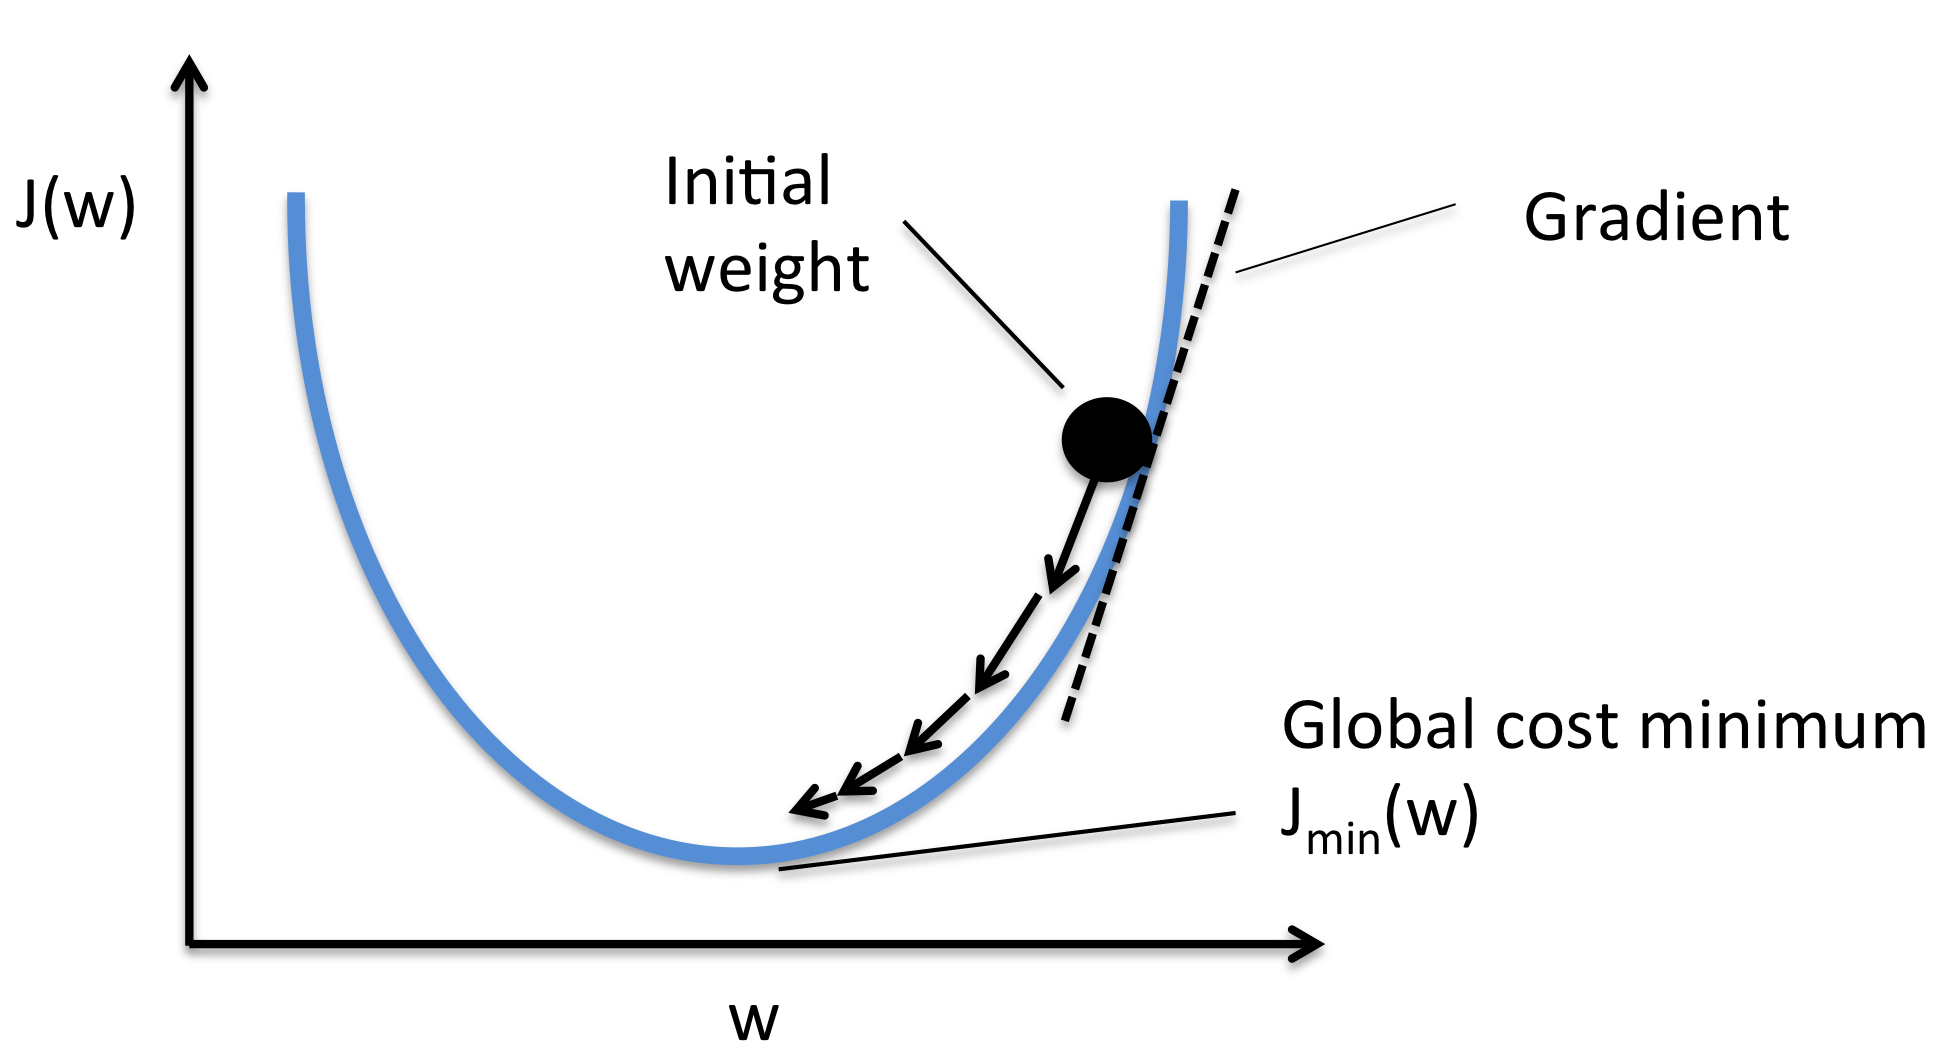
\includegraphics[scale=.15]{image/gradientdescent}
    \end{center}
    \caption{Gradient descent}
    \label{fig:gradientdescent}
    \end{figure}
\end{center}
 
Ngoài ra, trong các ứng dụng quy mô lớn, khi mà tập dữ liệu huấn luyện trở nên rất lớn, ví dụ như hàng triệu ảnh, thì sẽ rất lãng phí nếu chúng ta tính toán hàm mất mát trên toàn bộ tập dữ liệu trong mỗi lần cập nhật trọng số. Các tiếp cận đơn giản cho vấn đề này là chia ra các đợt (batchs) để huấn luyện. Chẳng hạn, mỗi batchs chúng ta sẽ tính toán trên 2 ảnh và thực hiện việc cập nhật trọng số, rồi sẽ thực hiện tiếp trên các batchs còn lại của tập dữ liệu huấn luyện. Phương pháp này chính là \textit{mini-batch gradient descent}
\end{enumerate}

\section{Convolutional neural network}
\subsection{Phân tích}

Với mạng nơ-ron truyền thống, vấn đề trong việc giải quyết các nhiệm vụ trong lĩnh vực thị giác máy tính là một ảnh khiêm tốn cũng sẽ chứa một lượng thông tin khổng lồ.\\

Một ảnh với kích thước 620x480 sẽ có 297600 pixel. Nếu mỗi pixel là mỗi input của một mạng full-connected, mỗi nơ-rơn sẽ có 297600 trọng số. Với một ảnh full HD 1920x1080, một nơ-ron sẽ có 2,073,600 trọng số. Mặc khác, chúng ta có nhiều lớp, do vậy, lượng trọng số chúng ta phải xác định sẽ rất khổng lồ.

\subsection{Kiến trúc cơ bản}
Ý tưởng cơ bản của Convolution neural network(CNN) dựa trên một khái niệm trong sinh học, là vùng thụ cảm (receptive field), hoạt động giống như một cảm biến, chúng nhạy cảm với một số loại kích thích, ví dụ như các cạnh, góc, kiến trúc của các vật thể trong ảnh.\\

ConvNets cũng tương tự như một mạng nơ-ron truyền thống, chúng được cấu thành từ nhiều nơ-ron có khả năng học các trọng số và biases. Mỗi nơ-ron nhận vào một đầu vào(vd:như matrix pixels), thực hiên một phép nhân ma trận sau đó giá trị này sẽ là đầu vào của một hàm phi tuyến. Chức năng sinh học có thể được mô hình hóa bằng máy tính nhờ phép toán chập (convolution operation) .\\

Một CNN thường gỉa định rằng đầu vào là ảnh, điều đó cho  phép chúng mã hóa những đặc tính quan trọng của một bức ảnh nhờ vào kiến trúc của nó. Không giống như mạng neuron thường, các lớp của một ConvNet gồm các nơ-ron được sắp xếp theo 3 chiều: cao, rộng và dài. Thêm vào đó, các nơ-ron trong một lớp chỉ kết nối đến một vùng nhỏ của lớp trước nó, thay cho việc các nơ-ron lớp sau kết nối một cách đầy đủ với các nơ-ron lớp trước như trước đây.\\

Mỗi lớp thực chất chuyển một đầu vào có 3 chiều thành một kết quả 3 chiều với một vài hàm có thể có tham số hoặc không. Phép toán chập của một bức ảnh f và một bộ lọc dưới dạng matrix g được định nghĩa như sau:

\begin{center}
	\begin{equation}
	 h[x; y] = f[x; y] * g[x; y] = \displaystyle \sum_{n}\displaystyle \sum_{m}f[n; m]g[x - n; y - m]
	\end{equation}
\end{center}
\begin{center}
    \begin{figure}[H]
    \begin{center}
     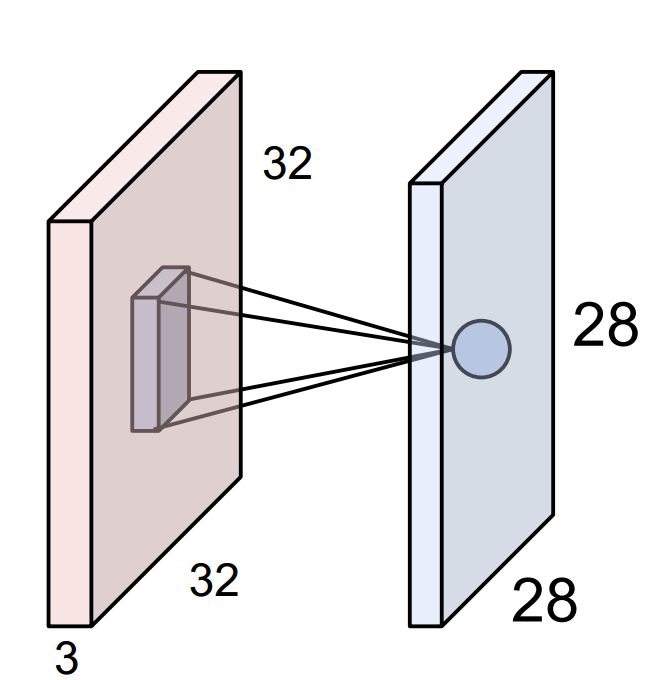
\includegraphics[scale=.5]{image/neuronView.PNG}
    \end{center}
    \caption{}
    \label{fig:conv_operation}
    \end{figure}
\end{center}

Phép toán trên giống như một neuron với bộ lọc g nhìn vào một vùng nhỏ f của lớp trước nó và cho ra một giá trị h tại tọa độ x,y. Kích thước của vùng thụ cảm bị thay đổi bởi kích thước của bộ lọc. Cho bộ lọc chạy dọc theo 2 chiều của bức ảnh để sinh ra một ma trận mới là h. Nó thường được gọi là các trích xuất đặc điểm(feature map) hoặc activation map sau khi h đi qua hàm activation). Nếu ảnh f không có đệm( padding) thì kích thước đầu ra sẽ giảm sau mỗi lần tính phép chập.\\


Một tập hợp các bộ lọc(convolution filter) sẽ tạo thành một lớp convolutional của mạng nơ-ron. Ma trận chứa dữ liệu của filters chính là các trọng số và sẽ được huấn luyện sử dụng các thuật toán học máy. Và các thao tác tích chập này (convolution) sẽ thay thế cho thao tác nhân ma trận ở mạng neuron thông thường. Giá trị đầu ra của lớp convolution giống như hình hộp chữ nhât với chiều sâu bằng số filter. Chiều rộng và chiều cao của khối sẽ giảm so với kích thước ban đầu nếu không được padding.\\

Bởi vì cùng một filter sẽ được sử dụng cho tất cả các phần của bức ảnh, do đó số lượng trọng số sẽ giảm xuống rất nhiều so với mạng fully-connected. Những nơ-ron của một lớp convolutional đều dùng chung một bộ tham số và chúng chỉ kết nối đến một vùng tương ứng trên đầu vào.

\begin{center}
    \begin{figure}[H]
    \begin{center}
     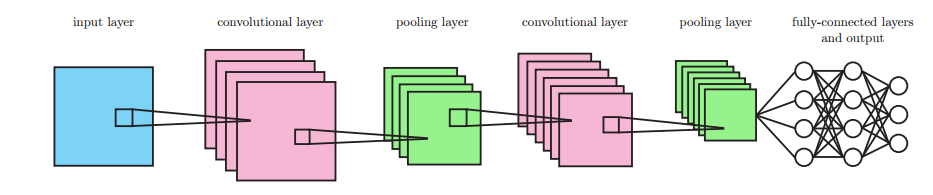
\includegraphics[scale=.5]{image/CNNexample.PNG}
    \end{center}
    \caption{An example of a convolutional network}
    \label{fig:cnn}
    \end{figure}
\end{center}

Ảnh trên là một ví dụ về một mạng ConvNet. Giải thuật lan truyền ngược đã  thảo luận ở trước vẫn được áp dụng. Về mặt lý thuyết, thì những lớp gần input sẽ học được những đặc tính đơn giản của bức ảnh như các cạnh, góc và các lớp sau sẽ tổng hợp những đặc tính học được từ lớp trước để nhận ra những hình dạng phức tap hơn được mô tả như hình bên dưới

\begin{center}
    \begin{figure}[H]
    \begin{center}
     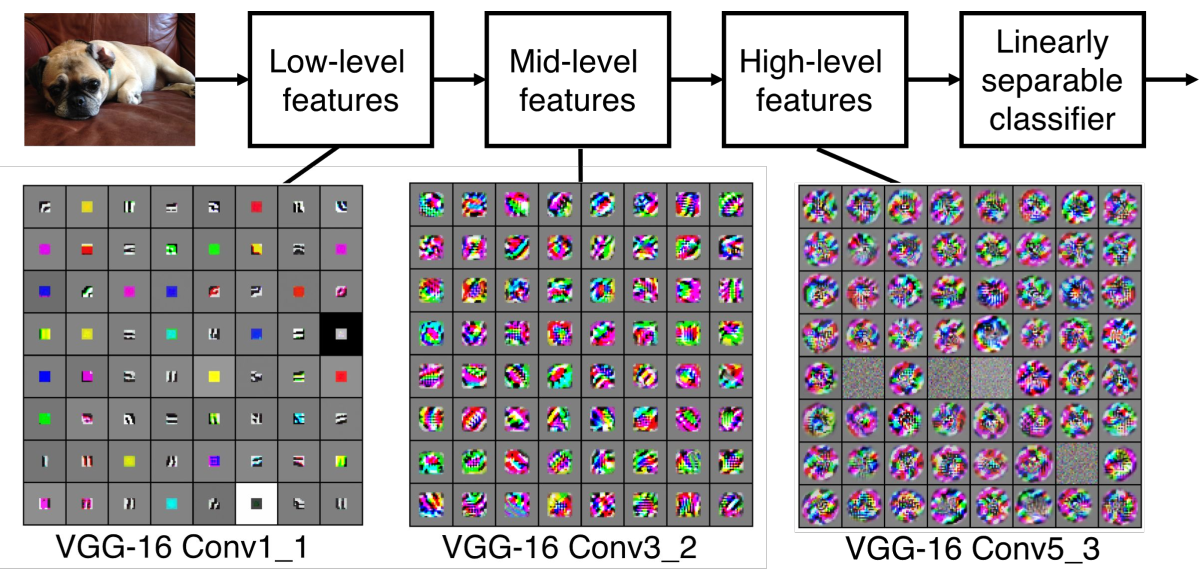
\includegraphics[scale=.5]{image/featureLearning.PNG}
    \end{center}
    \caption{Visualizing the content at each layer}
    \label{fig:visualize_cnn}
    \end{figure}
\end{center}


\subsection{Pooling và stride} 
Với một mạng dùng để phân loại ảnh, một điều cần thiết là nên giảm kích thước của activation map.Thường thì mạng nằm ở nằm sâu phía trong thì cần ít thông tin về đặc tính vị trí, hình dạng mà cần nhiều bộ lọc để có thể nhận ra những mẫu ở mức high-level. Người ta giảm chiều dài và chiều rộng của input volume bằng cách cho nó qua các lớp pooling hoặc tăng bước đi (stride).\\

Với pooling việc giảm kích thước của input volume sẽ giúp giảm số lượng tham số và thời gian tính toán của mạng, qua đó giúp ta kiểm soát hiện tượng over-fitting. Pooling layer tính toán độc lập trên mỗi activation map của một input volume khiến output volume sẽ có cùng chiều sâu với input nhưng chiều rộng với chiều cao đã giảm. Nhưng pooling có thể làm mất đi những thông tin về sự liên hệ đến hình dạng giữa những phần của các mẫu. Phương pháp pooling thông thường là max-pooling đơn giản nó chỉ cho ra giá trị lớn nhất trong hình chữ nhật tương ứng với kích thước bộ lọc mà nó chọn.\\
\begin{center}
    \begin{figure}[htp]
    \begin{center}
     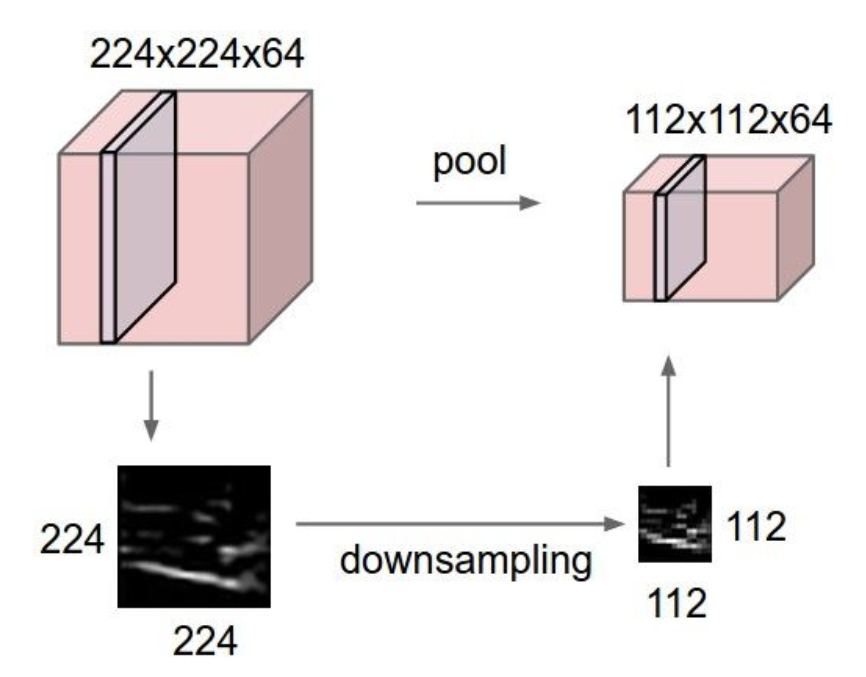
\includegraphics[scale=.5]{image/pooling}
    \end{center}
    \caption{An example of a pooling operation}
    \label{ref_chapter3_cnn}
    \end{figure}
\end{center}

Một cách khác để giảm input volume là tăng bước đi (stride) trong phép chập (vd: stride bằng 1 thì ta sẽ dich chuyển filter tại 1 pixel 1 lần). Theo nhiều nghiên cứu thì người ta không dùng pooling layer mà không mất đi độ chính xác bằng cách chỉ sử dụng nhưng bước đi lớn hơn tại mỗi phép chập.

\subsection{Additional layers}
Lớp convolutional thường có một hàm activation là hàm phi tuyến, như ReLu, thông thường nó được tách ra thành một lớp riêng nằm giữa lớp convolutional và lớp pooling.
Lớp cuối cùng của một ConvNet thường là fully-connected layer.\\

Một lớp fully-connected có thể lấy ra được những liên hệ thú vị của các phần từ input mà lớp convolutional không thể làm được. Tuy nhiên, để lớp này làm việc hiểu quả thì input cho nó phải là một volume có kích thước nhỏ thôi. Pooling và stride như phân tích ở trên sẽ làm giảm kích thước cho phù hợp, rồi mới đưa vào cho lớp này xử lí. Một số mạng không dùng đến fully-connected layer gọi là fully convolutional network (FCN).\\

Nếu mạng sử dụng cho image classification. Thì phần mạng phía trước fully-connected layer hoạt động giống như một bộ lọc, biểu diễn những đặc tính quan trọng, và khi đến lớp này chúng sẽ tổng hợp lại để đánh giá xem input là thuộc mẫu nào.
\begin{center}
    \begin{figure}[htp]
    \begin{center}
     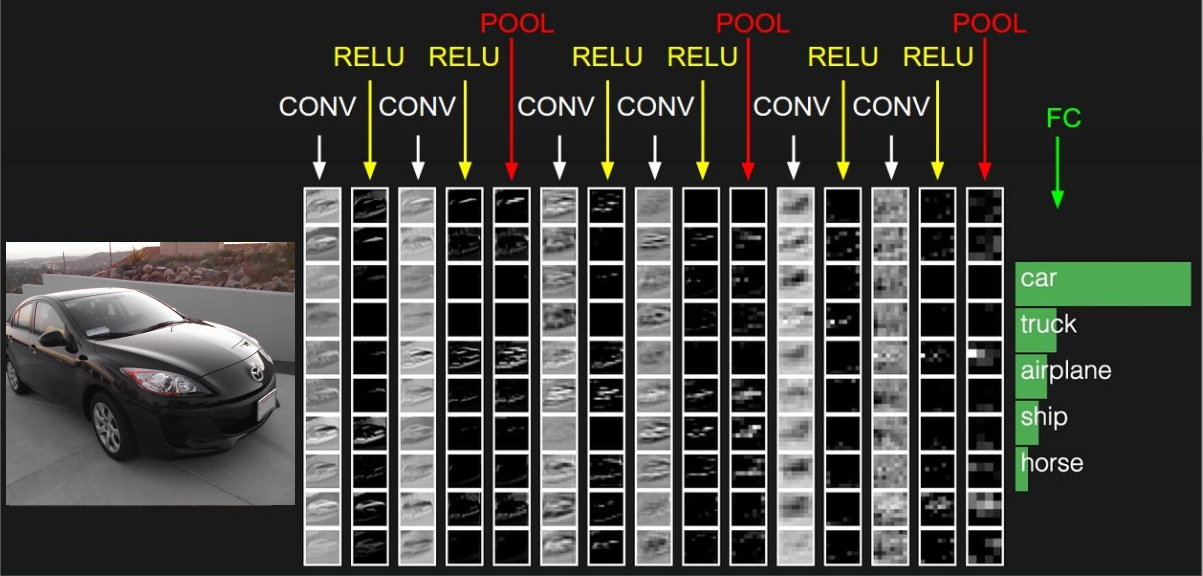
\includegraphics[scale=.5]{image/imageClass}
    \end{center}
    \caption{Classifying an image using a ConvNet}
    \label{ref_chapter3_cnn}
    \end{figure}
\end{center}
\subsection{Regularization}
Để can thiệp vào hiện tượng overfitting người ta thường đưa thêm những ràng buộc hoặc thông tin cho một hệ thống tự học. 
Một cách khá thông thường được sử dụng trọng mạng neuron để giới hạn khả năng của mô hình là thêm một tham số mới vào hàm đo độ lỗi hay hàm mục tiêu, ở đây ta định nghĩa hàm K\cite{DLbook}
\begin{center}
	\begin{equation}
	 K(\Theta;X;y) = J(\Theta;X;y) + \alpha\Omega(\Theta)
	\end{equation}
\end{center}
Nếu $\alpha = 0$ thì sẽ không có chính quy hóa, $\alpha$ càng lớn thì tăng chính quy hóa. Thường hàm K sẽ là hàm lỗi và nếu $\alpha$ lớn nó sẽ khiến cho giá trị của các trọng số học được nhỏ.\\

Dùng chung tham số trong ConvNet cũng là một ví dụ khác của chính quy hóa.
Một cách khác cũng khá phổ biến là dropout. Nó sẽ ngẫu nhiên bỏ đi một số neuron trong quá trình huấn luyện bằng việc thiết lập những giá trị tại đây là 0, nó sẽ tạo ra một mạng khác một ít so với ban đầu. Điều này sẽ khiến cho hệ thống không phụ thuộc quá nhiều vào số kết nối hoặc mỗi neuron, do đó giúp tính toán hiệu quả hơn. Trong ConvNet thì dropout thường sử dụng ở fully-connected layer.\\

Overfitting còn có thể được giảm bằng cách tăng số lượng của tập dữ liệu huấn luyện. Nếu không thể thu thập thêm được các mẫu thực tế cho tập huấn luyên, thì có thể tăng bằng cách sinh ra những mẫu mới từ những mẫu đã có, phương pháp này gọi là data augmentaion. 
Với việc phân loại bằng ConvNet, thì ta có thể sửa đổi một ít từ ảnh đầu vào sao cho việc nhận biết đối tượng thuộc lớp này không bị ảnh hưởng Vd: Ảnh có thể xoay các hướng khác nhau , tạo nhiễu...

\begin{comment}
\section{Microsoft Kinect và RGB-D image}
\subsection{Kinect camera}
\begin{center}
    \begin{figure}[htp]
    \begin{center}
     \includegraphics[scale=.5]{image/kinect}
    \end{center}
    \caption{Microsoft Kinect}
    \label{ref_chapter3_RGBD}
    \end{figure}
\end{center}

Kinect được ra mắt vào năm 2010, dữ liệu lấy được từ kinect bao gồm cả đặc tính về kích thước cũng như hình dạng. Điều này khiến cho nó là công cụ tiện lợi, được sử dụng trong nhiều lĩnh vực liên quan đến thị giác máy tính cả trong nghiên cứu lẫn công nghiệp\cite{kinect}.\\

Kinect có một máy ảnh màu và một bộ phát hồng ngoại (infrared (IR) emitter). Chúng có thể lấy được ảnh màu và độ sâu (depth) tại mỗi điểm ảnh (pixel). Dữ liệu này chứa thông tin về hình dạng và kích thước hình học, cho phép chúng ta giải quyết những vấn đề mà chỉ với ảnh màu thôi là không đủ.\\

Ảnh màu được tạo ra từ máy ảnh RGB. Độ sâu sẽ được ước đoán bằng cách dùng bộ phát hồng ngoại và máy ảnh, khi ở ngoài trời thì ước đoán giá trị độ sâu bị ảnh hưởng rất nhiều nên thiết bị này thường được sử dụng trong phòng là chủ yếu.
\end{comment}

\subsection{Lớp Unpooling và lớp Deconvolution}
\begin{enumerate}
\item \textbf{Unpooling}: Trong mạng convolution, thì lớp max-pooling sẽ không thể thực hiện ngược lại, nghĩa là từ kết quả đạt được khi thực hiện lớp max-pooling, chúng ta không thể có lại được giá trị đầu vào. Tuy nhiên, chúng ta có thể xấp xỉ giá trị này bằng cách ghi lại các vị trí lớn nhất của mỗi vùng khi thực hiện max-pooling. Trong quá trình thực hiện unpooling, dựa vào vị trí được khi nhận, ta sẽ bảo toàn được cấu trúc của giá trị đầu vào. Hình \ref{fig:unpooling} thể hiện rõ và chi tiết quá trình unpooling. 


\begin{center}
    \begin{figure}[H]
    \begin{center}
     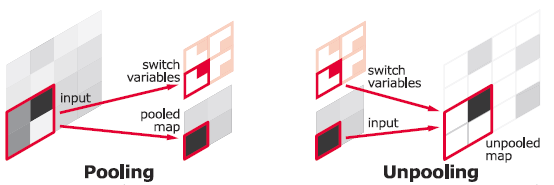
\includegraphics[scale=.6]{image/unpooling}
    \end{center}
    \caption{So sánh quá trình thực hiện max-pooling và un-pooling}
    \label{fig:unpooling}
    \end{figure}
\end{center}

\item \textbf{Deconvolution}: Lớp deconvolution hay còn có tên gọi khác là transposed-convolution, nhằm để tăng kích thước của giá trị đầu vào. Bằng cách thực hiện padding đủ lớn giá trị đầu vào, ta sẽ thực hiện được phép convolution lên giá trị mới này và và đạt được kết quả với kích thước lớn hơn.  


\begin{center}
    \begin{figure}[H]
    \begin{center}
     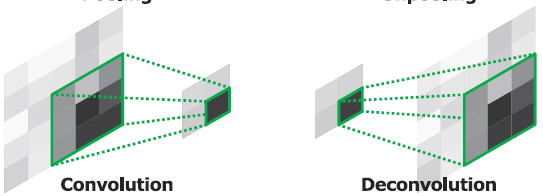
\includegraphics[scale=.6]{image/deconv}
    \end{center}
    \caption{So sánh quá trình thực hiện convolution và deconvolution}
    \label{fig:unpooling}
    \end{figure}
\end{center}


\end{enumerate}

% https://towardsdatascience.com/review-deconvnet-unpooling-layer-semantic-segmentation-55cf8a6e380e
 

\subsection{Biểu diễn ảnh RGB-D}
Ảnh RGBD là một tổ hợp của 3 kênh màu (đỏ,xanh lá cây và xanh dương) và thêm một kênh dữ liệu mới là độ sâu (depth data). Kênh màu có thể được biểu diễn bằng một ma trận của những số nguyên có 8 bit tương ứng từ 0 đến 255 nên nó biểu diễn được 256 màu tại mỗi điểm ảnh.\\

Độ sâu lại biểu diễn bằng một ma trận của những số nguyên có 16 bit nhưng thực tế nó chỉ dùng có 11 bit.
Kinect định giá trị của độ sâu trong khoảng từ 1 đến 10.000 giá trị đơn vị là milimet (1 đến 10.000mm).\\

Nhưng dữ liệu từ Kinect gặp phải một số vấn đề. Ảnh màu lẫn dữ liệu độ sâu đều có nhiễu. Bên cạnh đó cũng cần phải hiệu chỉnh lại những cái máy ảnh để tổng hợp ảnh màu và độ sâu sao cho chính xác.\\

Bức ảnh có thể có độ phân gải là 640x480 hoặc 1280x1024. Cả 2 độ phân giải này đều biểu diễn nhiễu về màu. Tương tự thì độ sâu cũng bị nhiễu và có những điểm ảnh lại không có được thông tin chiều sâu. Việc thiếu hụt này là do máy ảnh và bộ phát hồng ngoại nằm ở các vị trí khác nhau.\\

Viêc cần thiết là cần tiền xử lí lại dữ liệu bằng các phương pháp xử lí ảnh.


\section{ResNet}

Deep residual networks là một trong một những mô hình thể hiện sự đột phá trong lĩnh vực thị giác máy tính cũng như học sâu trong thời gian gần đây. Resnet có thể giúp huấn luyện những mô hình có số lượng layer rất lớn lên đến hàng trăm layer mà vẫn đạt được hiệu suất rất tốt. Với một lợi thế đáng kể như vậy, nó đã giúp cho nhiều ứng dụng thị giác máy tính có thể phân loại ảnh tốt hơn, điển hình là phát hiện đối tượng.\\

Tuy nhiên số layer càng lớn thì  mô hình càng dễ có xu hướng sẽ quá khớp (overfitting) với dữ liệu. Chúng ta có thể thấy xu hướng theo thời gian các mô hình ngày càng có số lượng layer tăng lên đáng kể, từ sau kiến trúc AlexNet thì các mô hình về sau đã có độ sâu tăng lên, AlexNet chỉ có 5 convolutional layers, VGG có 19 layers và GoogleNet có đến 22 layers. \\

Tăng số layer của một mô hình không đơn giản là xếp các layer chồng lên nhau, nếu chỉ xếp chồng lên đơn giản như vậy thì mô hình sẽ không hoạt động hiệu quả. Các mạng sâu rất khó để huấn luyện vì có thể sẽ gây ra hiện tượng triệt tiêu gradient trong quá trình backpropagation. Kết quả là khi mạng đi sâu thì hiệu suất dường như bị bão hòa và có xu hướng giảm xuống. Như theo hình \ref{fig:resnet_layer}, với số layer nhiều hơn, ta luôn nhận được lỗi trong quá trình huấn luyện cũng như lỗi trong quá trình đánh giá là lớn hơn.\\

\begin{center}
    \begin{figure}[H]
    \begin{center}
     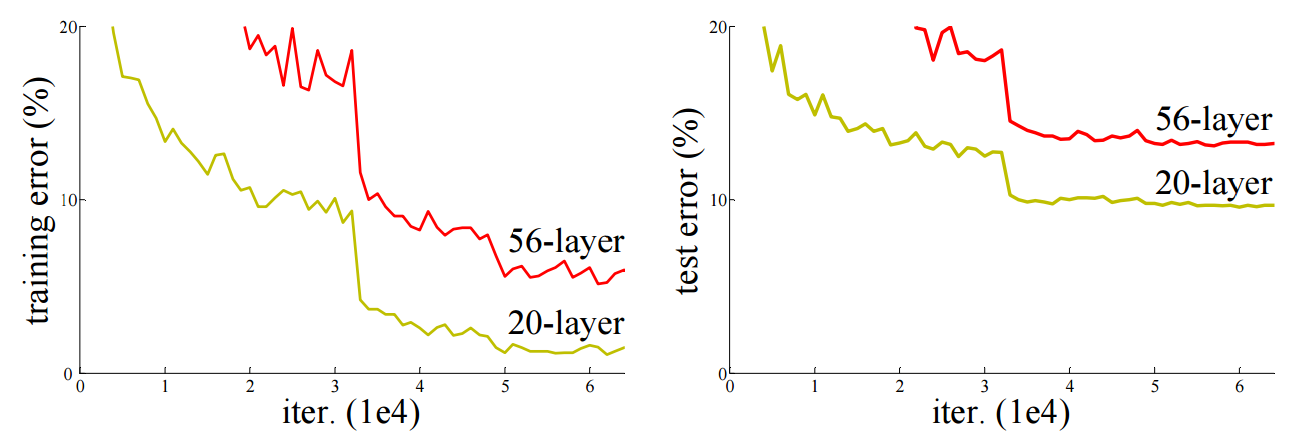
\includegraphics[scale=.25]{image/chapter3_resnet_compare}
    \end{center}
    \caption{Tăng số layer làm cho hiệu suất của mô hình giảm}
    \label{fig:resnet_layer}
    \end{figure}
\end{center}


Ý tưởng chính của Resnet là tạo ra một "identity shortcut connection" để có thể bỏ qua một hoặc nhiều layers, nếu như những layer đó đang bị triệt tiêu gradient, theo hình \ref{fig:resnet_block}.Các layers xếp chồng lên nhau, không làm cho hiệu suất của mạng bị suy giảm, do đã có các shortcut connection. Hiện nay, Resnet đã trở nên phổ biến, kiến trúc của nó được nghiên cứu rất nhiều và đã có khá nhiều những kiến trúc mới dựa trên Resnet.

\begin{center}
    \begin{figure}[H]
    \begin{center}
     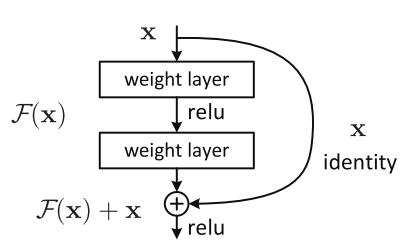
\includegraphics[scale=.5]{image/chapter3_resnet_block}
    \end{center}
    \caption{Một block của residual networks.}
    \label{fig:resnet_block}
    \end{figure}
\end{center}



 




 
